\section{Experimental Setup}
\label{expSetup}

%%%%%%%%%%%%%%%%%%%%%%%%%%%%%%%%%%%%%%%%%%%%%%%%%%%%%%%%%%%%%%%%%%%%%%%%%%%%%%%%%%%%%%%%%%%%%%%%%%%%%%%%%%%%%%%
%Initiator: Ran Itay
%Last modified by: MM Devi, May 26 2017
%Comment: The detector section has been modified. MMdevi's changes are made in blue
%%%%%%%%%%%%%%%%%%%%%%%%%%%%%%%%%%%%%%%%%%%%%%%%%%%%%%%%%%%%%%%%%%%%%%%%%%%%%%%%%%%%%%%%%%%%%%%%%%%%%%%%%%%%%%%

The experimental setup of DIREXENO is described in this section. This setup is 
designed to measure the spatial and temporal properties of LXe scintillation. 
It consists of a modular design in order to extend its flexibility
to fulfill the requirement of any different future experiments. 

Four main building blocks constitutes of the full setup, a schematics 
of which, with the interfaces between them is shown in Fig.~\ref{fig:fullschematics}. 
The gas handling system, in normal working mode, drives the xenon from the detector through 
a purifier and cycles it back into the detector. The cryogenic system, liquefies the xenon and 
delivers it to the detector system. The detector system consists of a fused silica sphere that 
holds a small bubble of LXe target, and PMTs around the sphere. The supply of high voltage (HV) 
to the PMTs and the data readout are carried out through the 
data acquisition system (DAQ) system. 
These four building blocks are independent of each other construction wise, and can be 
replaced without altering features in the others. 

\begin{figure}[h]
\centerline{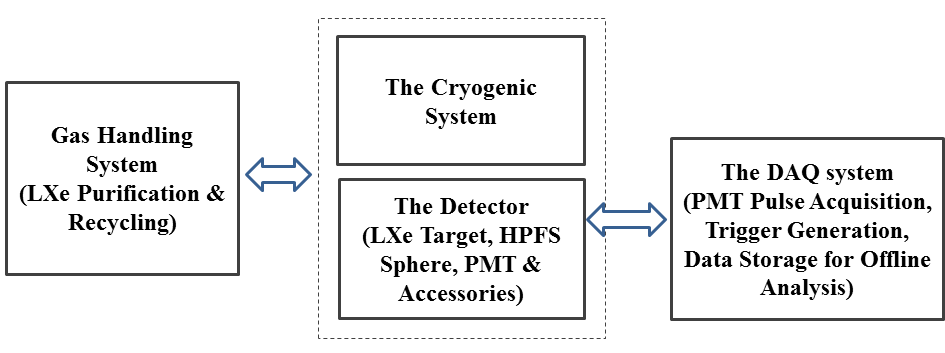
\includegraphics[width=0.8\linewidth]{WholeSys.png}}
\caption{A schematic of DIREXENO showing all the four building blocks of the system.}
\label{fig:fullschematics}
\end{figure}

The full assembly, shown in Fig.~\ref{fig:fulldet}, is held on three separate racks, 
one for the gas handling system, another to hold the cryogenic and the 
detector while the third one is assigned for the DAQ. The racks are joined using a 
100mm bar with shock absorbers on both sides. Some of the guidelines for the design of 
DIREXENO are based on~\cite{Giboni}.  

\begin{figure}[h]
\centerline{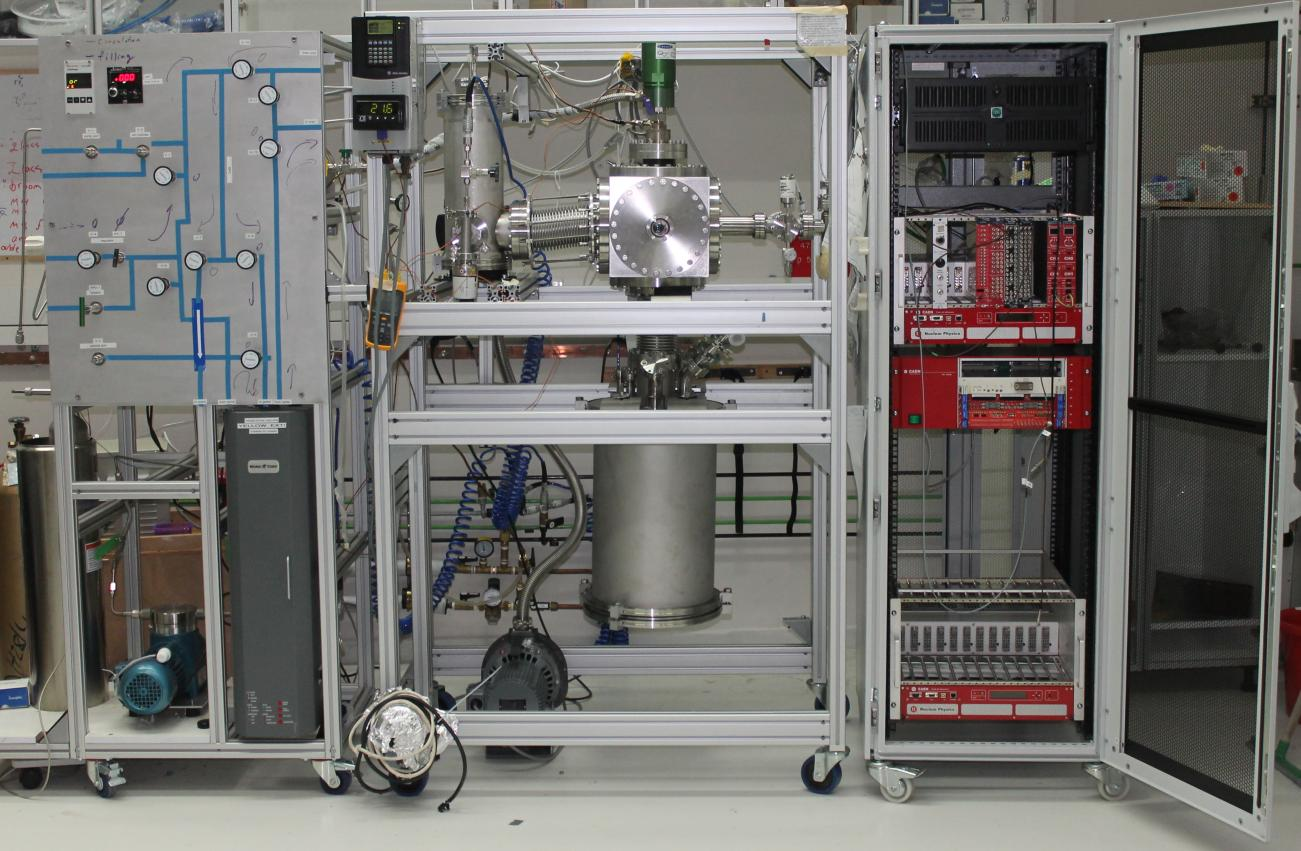
\includegraphics[width=0.8\linewidth]{FullDet.jpg}}
\caption{DIREXENO. On the left the purification system, in the middle the cryogenic and detector 
chamber, and on th right the Data acquisition system.}
\label{fig:fulldet}
\end{figure}

\subsection{Gas handling system}
\label{subsec:gas}

A typical LXe detector must keep a high level of purity. Careful selection and 
meticulous cleaning of all parts before mounting is needed, however it is not 
sufficient. The desired level of most detectors of impurity concentration is at 
the level of 1 ppb $O_2$ equivalent~\cite{Aprile:2009dv}. This is crucial to allow 
ionization electrons drift for several cm. To reach that level in a reasonable amount 
of time (several days instead of months), 
a continuous purification is needed. The gas handling system provides this process along 
with all gas handling operations such as filling and recuperation.

During purification mode, xenon is taken from the chamber (in liquid phase)
passes through a heat exchanger\footnote{GEA GBS100M-24 plate heat exchanger} 
where it is heated and vaporized. The xenon is forced 
by a KNF diaphragm pump into a hot getter\footnote{MONO-TORR
PS4-MT15-R-2} which cleans the xenon from most impurities. The xenon
also passes through an MKS Mass Flow Controller\footnote{MKS mass flow controller} (MFC), 
this allows monitoring and controlling the amount of xenon in the system. 

After the xenon is purified, it is delivered back to the cryogenic system 
through the heat exchanger, where the remaining gaseous xenon is 
liquefied before it continues back to the chamber. A schematic of this 
system is shown in fig.~\ref{fig:gasSchematic}.


%%%%%%%%%%%%%%%%%%%%%%%%%%%%%%%%%%%%%%%%%%%%%%%%%%%%%%%%%%%%%%%%%%%%%%%%%%%%%%%%%%
\begin{figure}[h]
\centerline{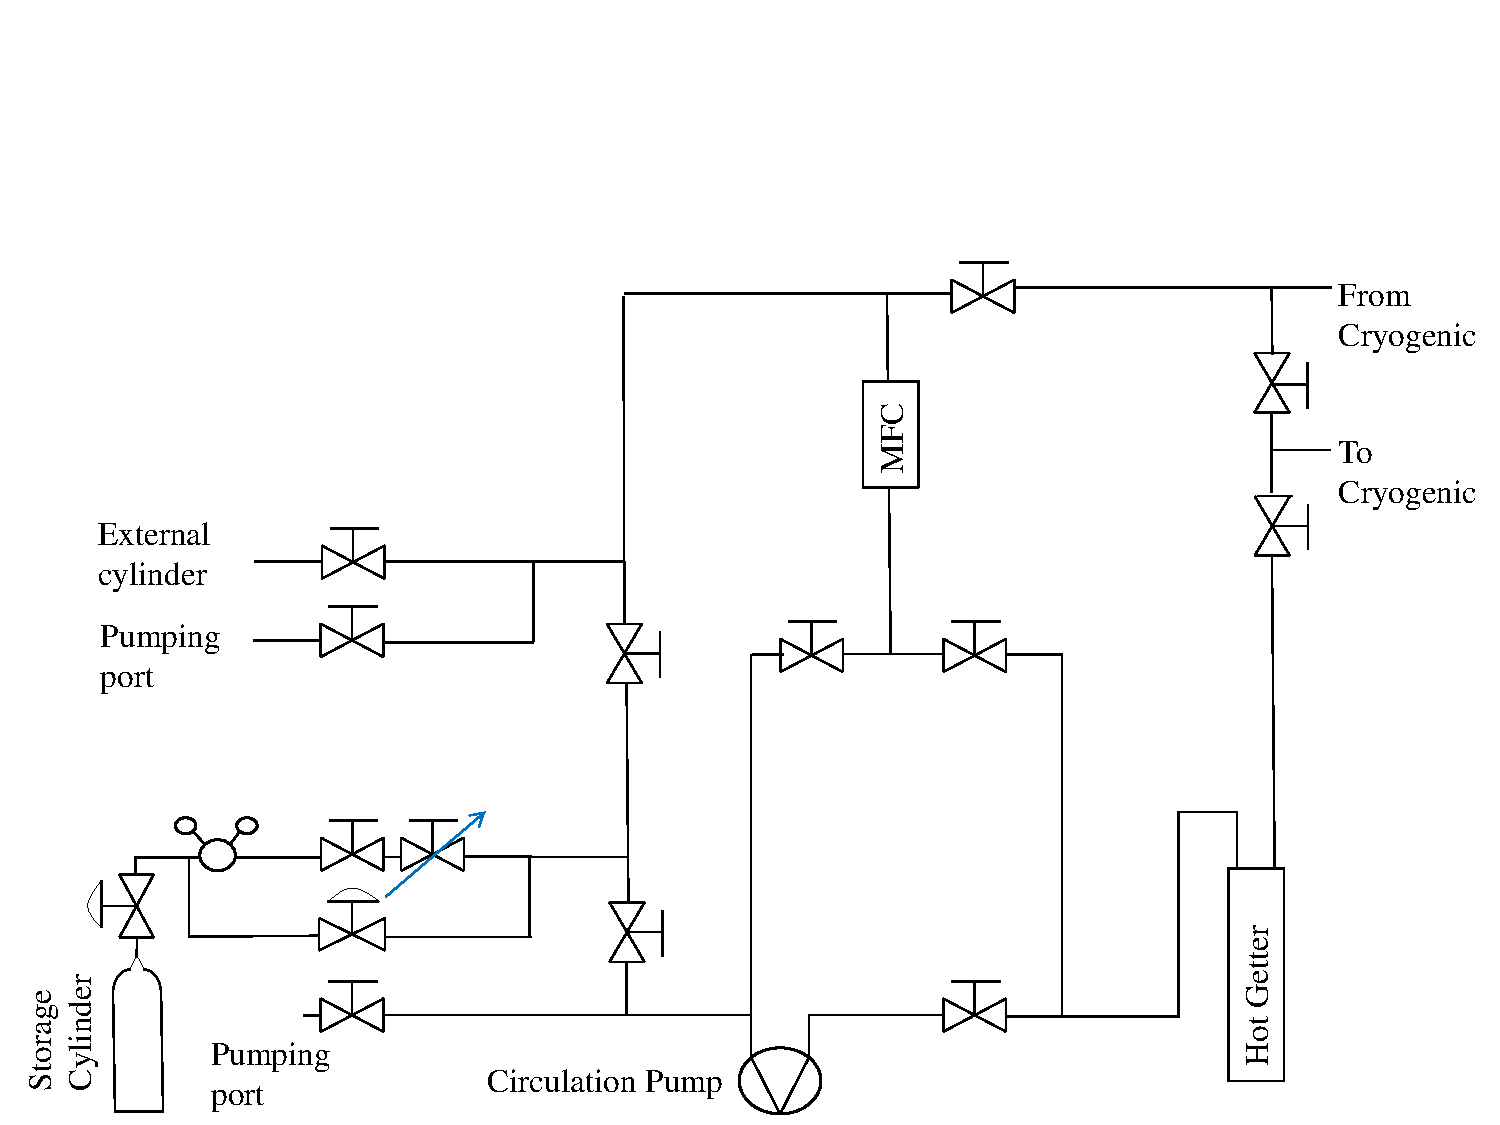
\includegraphics[width=0.75\linewidth]{GasSchematics.pdf}}
\caption{Schematics of the purification system. High pressure valves are indicated as 
valves with arcs. Needle valves are indicated as 
a valve with an arrow.}
\label{fig:gasSchematic}
\end{figure}
%%%%%%%%%%%%%%%%%%%%%%%%%%%%%%%%%%%%%%%%%%%%%%%%%%%%%%%%%%%%%%%%%%%%%%%%%%%%%%%%%%

\subsection{Cryogenic system}
\label{subsec:cryo}

Remote cooling is generally used in DM experiments due to background radiation
from the cooler to the detector. Although this is not of a great 
importance in our system, there still are several advantages of remote 
cooling such as: lowering acoustic noise from the cryo-cooler and 
flexibility to design changes. 
The cryogenic system is connected to the gas handling system on 
one side and to the detector chamber on another side. 
The cryogenic system is build such that replacing the cryo-cooler type 
(e.g., to PTR) requires just an adaptation to the top flange.


The system is made of two chambers, the outer vessel (OV) which holds 
the insulation vacuum, and the inner vessel (IV) that holds the xenon. In addition to the vacuum which prevents heat leakage due to diffusion and convection, the entire IV is covered by multi layer aluminized Myler to prevent heating via radiation. The CAD view of 
the design of the cryogenic system and a photo of the actual system are shown in Fig~\ref{fig:cryo}. 

%%%%%%%%%%%%%%%%%%%%%%%%%%%%%%%%%%%%%%%%%%%%%%%%%%%%%%%%%%%%%%%
\begin{figure}[h]
\centering
\begin{subfigure}[c]{0.25\textheight}
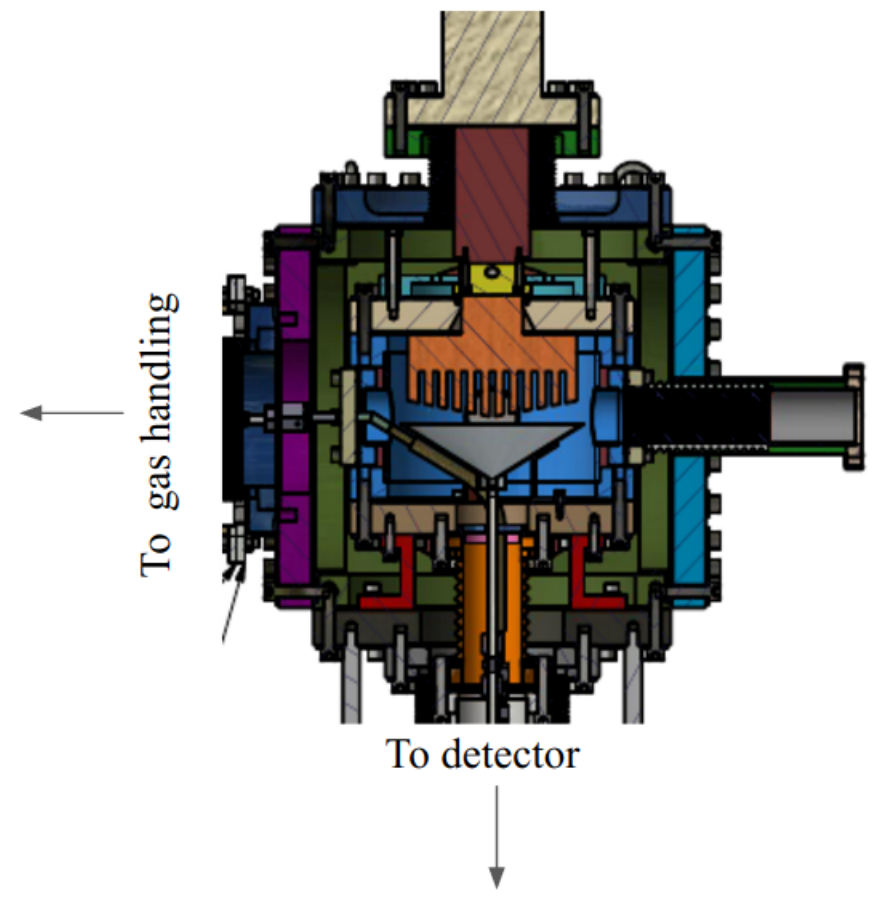
\includegraphics[width=\textwidth]{cryoMirror.png}
\end{subfigure}
\begin{subfigure}[c]{0.25\textheight}
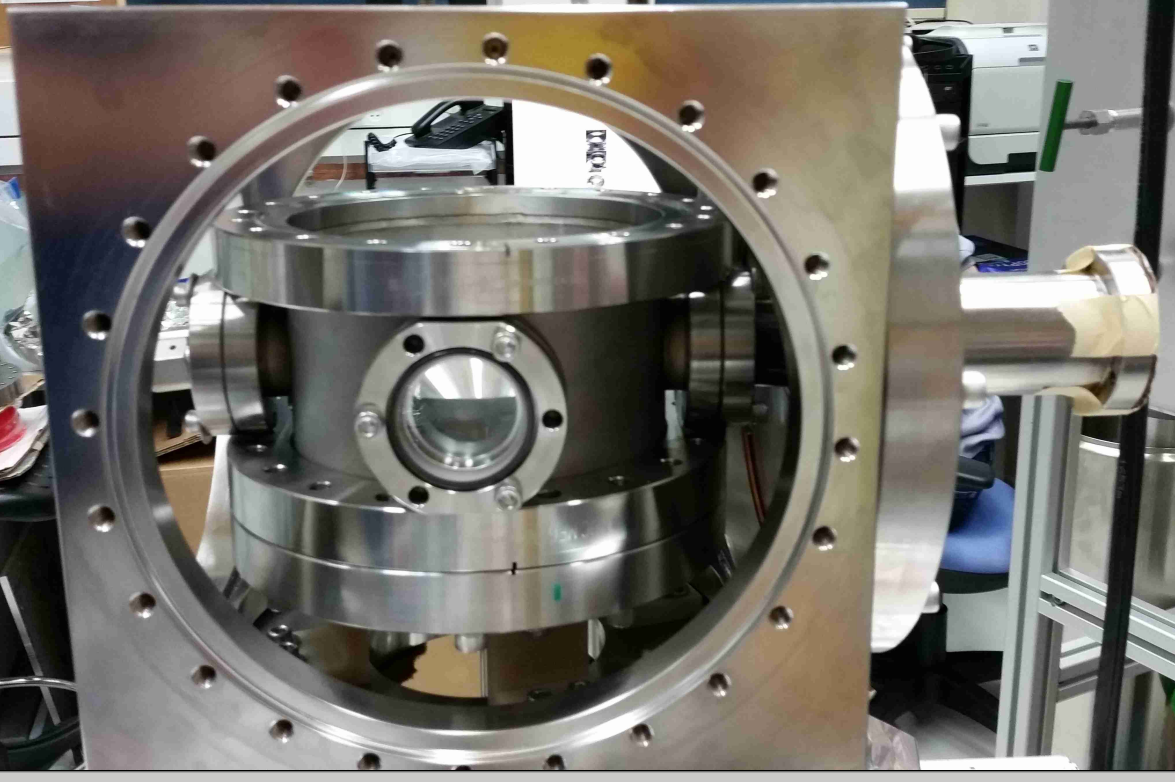
\includegraphics[width=\textwidth]{cryoOpenCrop.png}
\end{subfigure}
\caption{ CAD view of the cryogenic system(Left) and a picture of the cryogenic system (Right) . 
The cryogenic system. (Left) CAD design view, 
(right) picture of the actual system.
\label{fig:cryo}}
\end{figure}
%%%%%%%%%%%%%%%%%%%%%%%%%%%%%%%%%%%%%%%%%%%%%%%%%%%%%%%%%%%%%%%%

The OV is made of a 10" CF cube, with ports on all six faces (e.g., FT, pumping ports, 
view ports). This vacuum is shared with the detector one via a 6" CF flexible bellows.
The IV is made of 1.5" height cylinder with 6" CF flanges on the top and bottom parts of it, 
and it holds xenon inside. A 120~\,mm diameter cold finger is welded to the top flange of the IV, 
the inner part of the cold finger is made of long fins, therefore the surface area of it is bigger 
resulting in a better heat transport. The design of the cold finger is similar to the design 
of~\cite{xe100_instr2012}. The upper part of the cold finger is in thermal contact with the 
cryo-cooler~\footnote{QDrive 20BB 9p6 A 3 AYNBNCO} via a copper adapter. The copper adapter 
holds two $100\Omega$ pt resistor which are connected to a PID reader\footnote{cryo-con model 
18i Cryogenic Temp Monitor} for temperature measurements. A cartridge-heater 
is also inserted to the copper adapter for emergency heating in case xenon freezes on the 
cold finger. 

The cryo-cooler provides up to 70 W of cooling power, and is connected via a $4\frac{1}{2}$" 
flange to the OV top flange, and reaching the IV top flange. The common cryo-coolers used for 
xenon experiments work in maximal cooling mode permanently. The QDrive, instead, has 
temperature control allowing it vary the cooling power, which enables to set the temperature 
with fluctuations smaller then $0.1~\mathrm{^{\circ}C}$ on the cooler itself.

On the inner side of the bottom flange of the IV a thin 0.6~mm SS funnel is installed 
collecting all LXe drops from the cold finger, and delivering them to the  detector part. 
This flange is connected to the detector part, via a $3\frac{3}{8}$" flexible bellows. This 
bellows hosts two small pipes connected to the circulation system, and a third pipe coming 
from the funnel. All three pipes deliver LXe whereas the GXe is filling the bellows. The 
separation between the LXe coming from the gas handling system (clean) and the LXe coming 
from the cold finger (more impure) allows the filling of clean LXe to 
different parts of 
the detector. 

%%%%%%%%%%%%%%%%%%%%%%%%%%%%%%%%%%%%%%%%%%%%%%%%%%%%%%%%%%%%%%%%%%%%%%%%%%%%%%%%%%%%%%%%%%%%%%%%%%%%%%%%%%%%%%%%%%%%%%%%%%%%%%%%%%%%%%%%%%%%%%%%%%%%%%%%%%%%%
\subsection{The Detector}
\label{subsec:det}
 
The detector refers to the chamber and its inner assembly consisting 
mainly of an HPFS\footnote{High Purity Fused Silica. Corning HPFS 8655 material is used.} sphere that 
contains the liquid Xenon, the photomultiplier detectors around it and their accessories. 
This chamber is placed below the cryogenic system. 


%mmd{I feel 
%that when we say ``these two parts'', it might not be a clear statement. We may either skip what we describe entirely, 
%or might keep it as in the following.} \RanComment{agreed I think we can drop this , the paper is short enough so we don't need to detail where we describe what.}
%We describe the detector chamber and its interface to the cryogenic system in 
%section \ref{subsubsec:detchamber}. In section \ref{subsubsec:sphere} we discuss the assembly 
%%around the sphere.
%%%%%%%%%%%%%%%%%%%%%%%%%%%%%%%%%%%%%%%%%%%%%%%%%%%%%%%%%%%%%%%%%%%%%%%%%%%%%%%%%%%%%%%%%%%%%%%%%%%%%%%%
\subsubsection{The Detector Chamber}
\label{subsubsec:detchamber}

The detector chamber is built in a way that apart from the interface to the cryogenic system, it can 
be changed and modified easily for future experiments. The interface unit is built out of 2 flanges 
welded together via 7 tubes, which serve as service ports for electrical and other feedthroughs, 4 
with a $2 \frac{3}{4}/$ CF flange, and 3 with a $1\frac{1}{3}$ CF flange. 
The upper flange, ISO-K NW320, is part of the OV and shares the insulation vacuum of the cryogenic 
system, the bottom one , CF-8", is part of an IV for future detectors, and would hold xenon inside. 
For our experiment we modified the CF flange to fit also a $4\frac{5}{8}$" CF 
flange which we use.

The OV is made of a ISO-K 320NW nipple closed with a blank from the bottom, 
the height of the nipple is determined such that the maximal height of the whole 
apparatus is 190~\,cm, allowing the mobility of the detector through standard doors.
 
The $4\frac{5}{8}$" CF flange is connected to a closed vessel internally divided into 
two parts. This vessel serves as a xenon reservoir. The two parts of the vessel are connected 
to a the HPFS sphere (see subcse~\ref{subsubsec:sphere}) from above (inner part) and from below 
(outer part). LXe is circulated such that new LXe drips into the outer part and pumped from the 
inner one. This way the liquid level is controlled, and the sphere itself is always filled with LXe. 



%%%%%%%%%%%%%%%%%%%%%%%%%%%%%%%%%%%%%%%%%%%%%%%%%%%%%%%%%%%%%%%%%%%%%%%%%%%%%%%%%%%%%%%%%%%%%%%%%%%%%%%%%%%%%%%%%%%%%%%
\subsubsection{The Sphere}
\label{subsubsec:sphere}

The central component of the detector assembly is a hollow sphere 
which holds the LXe bubble. A spherical shell made of Corning HPFS 8655 with high transmittance is 
designed to hold the LXe target. Two invar tubes 
are connected to the HPFS sphere from the top and bottom with 
SS mini-CF flanges at the end, which allows \sout{the} circulation of xenon through 
the sphere. The technical design and image of the sphere are shown in Fig.~\ref{fig:sphere}. 
The bottom flange of the sphere is held using a brass holder to prevent 
force or torque applied on the sphere while mounting the detector. The 
brass holder is connected to a plate held from the top 8" flange, and is 
also used to align this plate at first installation. A set of 20 
PMTs\footnote{R8520-406 Hamamatsu 1" PMT, active area 20.5 mm $\times 20.5 mm$} 
are placed around the sphere to detect light emitted from the LXe.


%%%%%%%%%%%%%%%%%%%%%%%%%%%%%%%%%%%%%%%%%%%%%%%%%%%%%%%%%%%%%%%%%%%%%%
\begin{figure}[h]
\centering
\begin{subfigure}[c]{0.4\textheight}
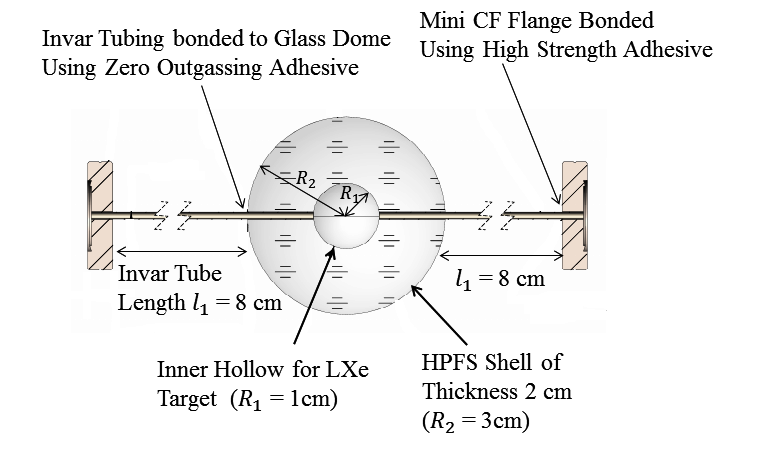
\includegraphics[width=\textwidth]{spheredesign1.png}
\end{subfigure}
\begin{subfigure}[c]{0.25\textheight}
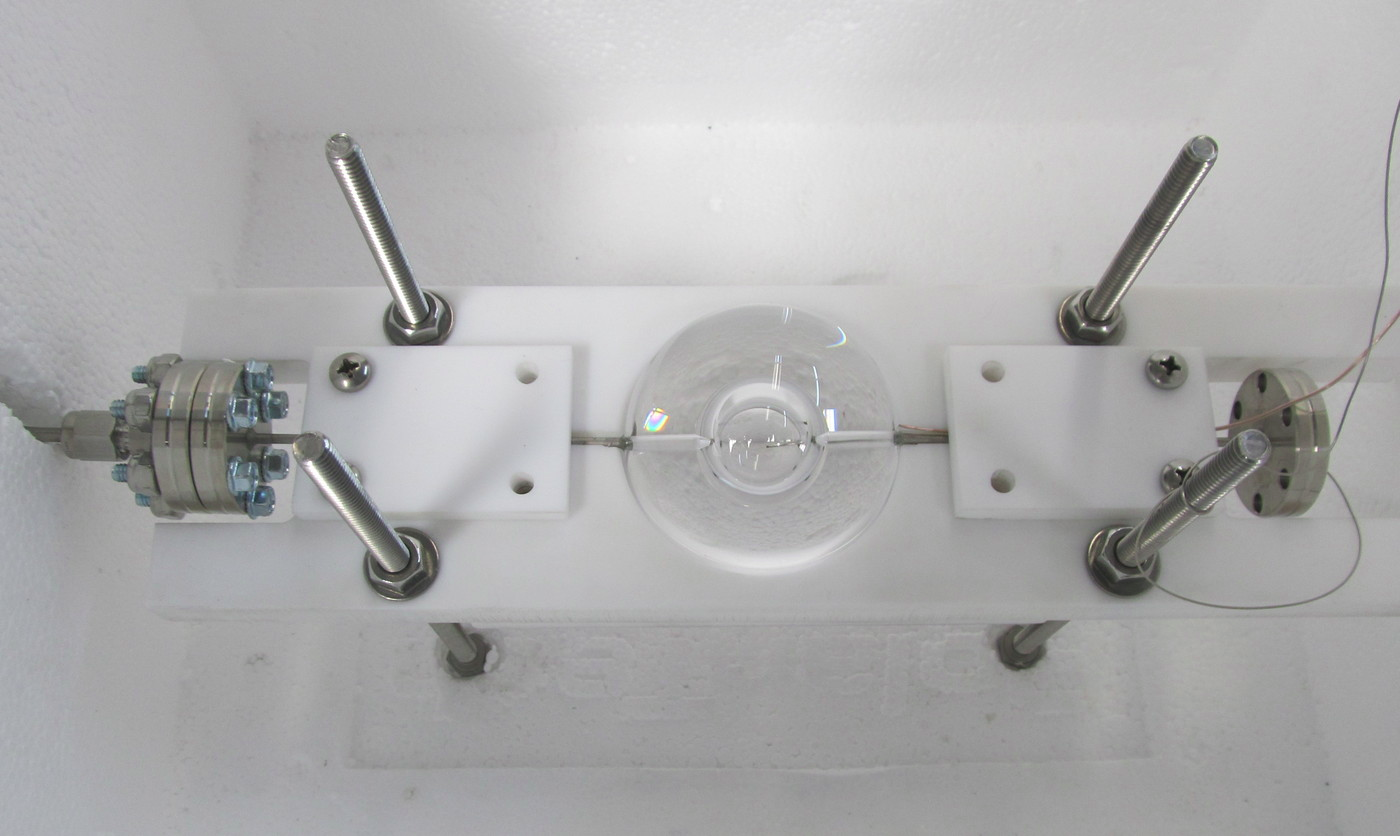
\includegraphics[width=\textwidth]{spherephoto.png}
\end{subfigure}
\caption{(Left)The technical design of the HPFS shell with invar tubing and mini CF flanges. 
(Right) The industrially manufactured HPFS shell.} 
\label{fig:sphere}
\end{figure}
%%%%%%%%%%%%%%%%%%%%%%%%%%%%%%%%%%%%%%%%%%%%%%%%%%%%%%%%%%%%%%%%%%%%%%%%



The LXe target bubble should not be too large in order to avoid double scatters. 
The HPFS shell should be large enough to reduce internal reflections, but not 
too large which would attenuate the scintillation light. The material of the 
shell should have a refractive index as similar to LXe as possible in order to 
have minimal diffraction from the original direction of the photons when they 
travel from the LXe target to the sphere. Corning HPFS 8655 is chosen as the shell 
material. The refractive index of HPFS 8655 is 1.575 at 185 nm (LXe R.I. 1.61). 
In Fig.~\ref{fig:hpfsRIcalibration} (left panel), are the refractive indexes at various wavelengths 
as provided on the HPFS 8655 fact sheet as well as a naive extrapolation to lower wavelengths 
which are relevant to us. 

\begin{figure}[h]
   \centering
   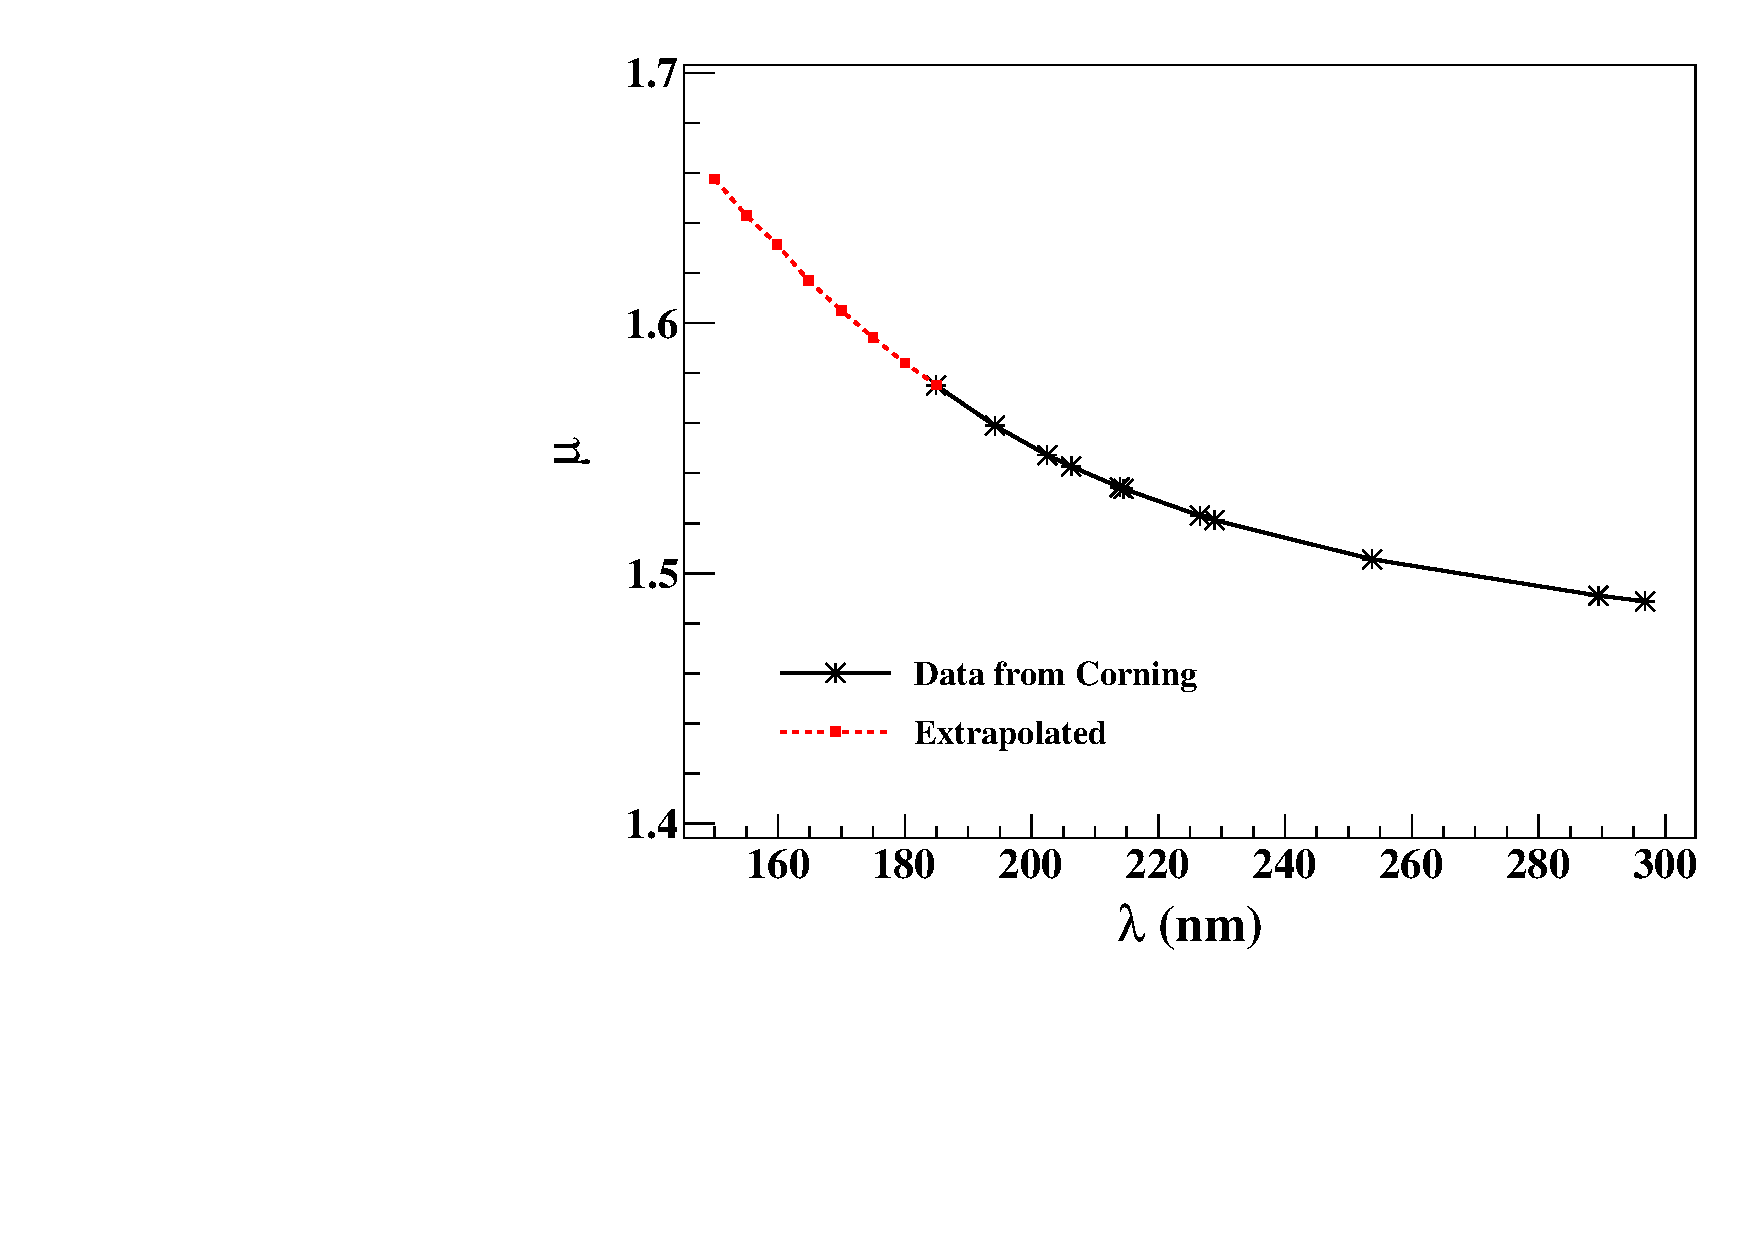
\includegraphics[width=0.48\textwidth]{RI-calibration.pdf}
    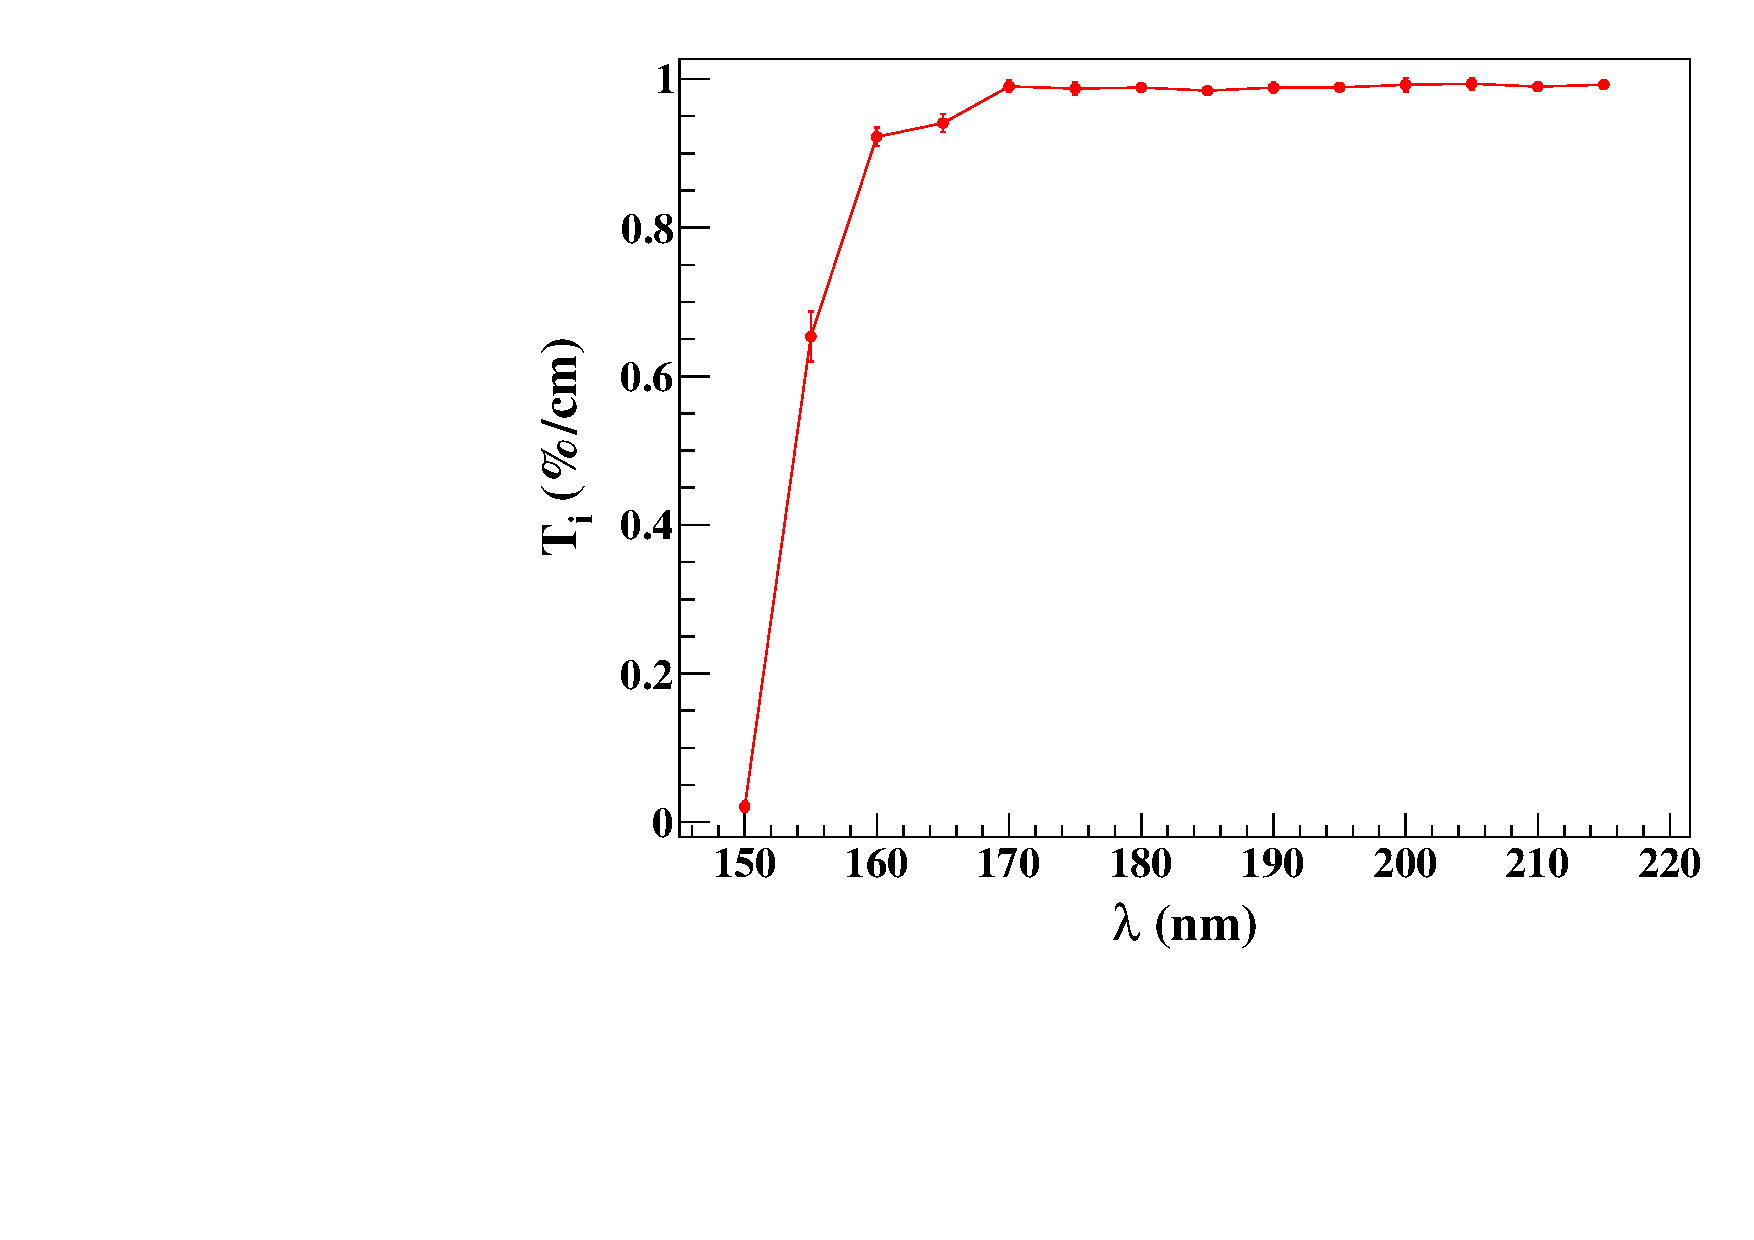
\includegraphics[width=0.48\textwidth]{IntTransmittance.pdf}
   \caption{The important characteristics of HPFS-8655. (Left) The refractive index as provided by corning and 
   extrapolated to relevant wavelength range. (Right) The internal transmittance ($T_{i}$).} 
   \label{fig:hpfsRIcalibration}
\end{figure}

The transmittance of the material is an extremely crucial parameter to optimize the 
dimension of the shell. Therefore, a sample of HPFS 8655 was tested for transmittance 
using a VUV monochromator. 
In fig.~\ref{fig:hpfsRIcalibration} (right panel), the measured 
transmittances (\%/cm) at (150 - 215)~\,nm are plotted. At 175~\,nm, the intrinsic transmittance 
of the sample about 98.7\%/cm.  


The dimension of the fused silica shell is optimized by studying the path of the 
scintillation photons using a GEANT4 based simulation~\cite{Agostinelli:2002hh}. 
The sources that will be used for exciting the xenon, and creating the supperradiance 
(signal) as well as the standard emission (background), will be $^{137} \mathrm{Cs}$ 
(662 keV) and $^{57} \mathrm{Co}$(122keV \& 136 keV) for ER and $^{241}$AmBe , 
D-D neutron generator, or neutron produced in an accelerator for NR . The mean 
free path for this energy is a couple of mm ($^{57} \mathrm{Co}$) and (0.5 - 3) 
cm ($^{137} Cs$).  The outer radius of the shell is 3 cm, while the inner radius of the 
hollow space that holds the LXe is 1 cm. 


Photons coming out of the system are detected by twenty R8520-406 PMTs with an 
active area of 20.5 mm $\times$ 20.5 mm each. 
The PMT are chosen to have a minimum 
quantum efficiency of 30\% at 178 nm. At an applied voltage of 900 
V the gain of these PMTs is ~ 2 $\times$ 10$^6$. A positive voltage divider, 
also manufactured by Hamamatsu,  is used to to provide high voltage to the PMTs. 
The PMTs are held with a special aluminum holder, coated with anti-reflection substance. 
The holder is made of two hemispheres hosting the PMTs in 3 rows all of them pointing to the 
center of the HPFS sphere. The PMTs are held only via their voltage--divider bases, while 
the bases are fixed with M2 PEEK screws. 
In Fig.~\ref{fig:pmtholder}, one of the holder--hemispheres with the 
PMTs is shown. A CAD schematic and a real view of the detector assembly are shown 
in In Fig.~\ref{fig:detector}.

%%%%%%%%%%%%%%%%%%%%%%%%%%%%%%%%%%%%%%%%%%%%%%%%%%%%%%%%%%%%%%%%%%%%%%%%%%%%%%%%%%%%%%%%%%%
\begin{figure}[h]
   \centering
   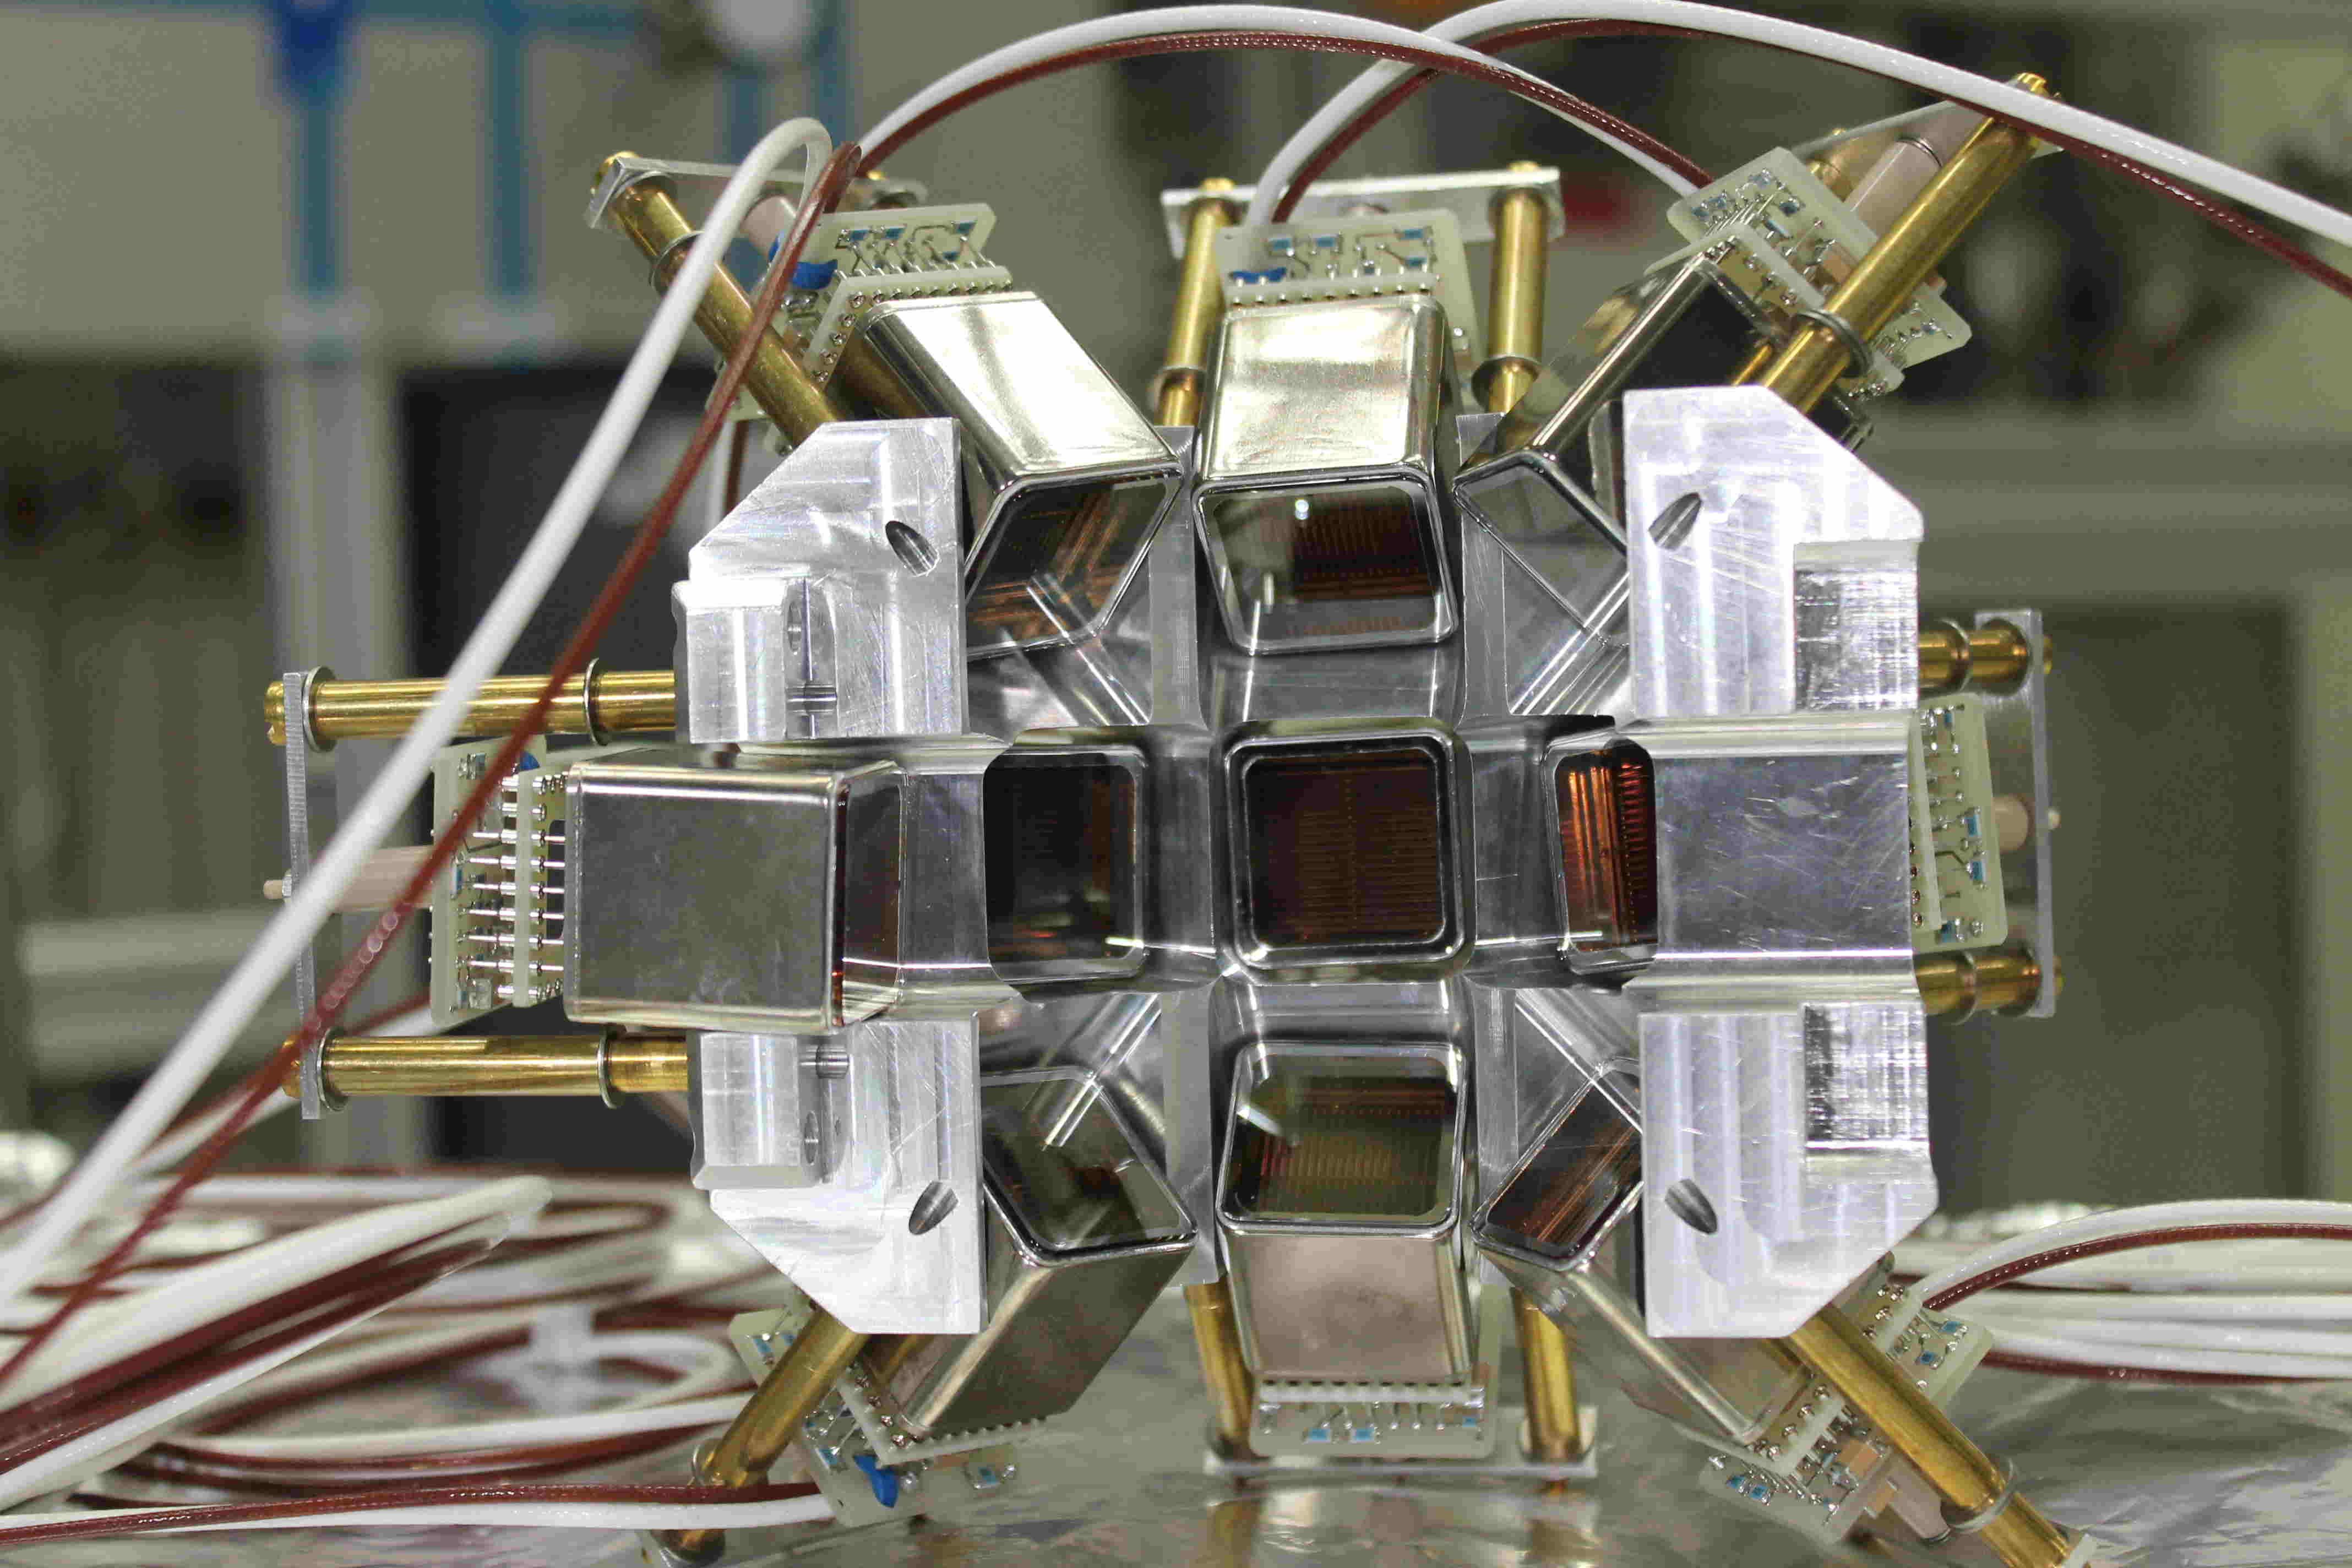
\includegraphics[width=0.5\textwidth]{PMTholder.JPG}
   \caption{A PMT holder--hemisphere. Two identical hemispheres are used to hold 
   the PMTS around the HPFS sphere.} 
   \label{fig:pmtholder}
\end{figure}
%%%%%%%%%%%%%%%%%%%%%%%%%%%%%%%%%%%%%%%%%%%%%%%%%%%%%%%%%%%%%%%%%%%%%%%%%%%%%%%%%%%%%%%%%%%

%%%%%%%%%%%%%%%%%%%%%%%%%%%%%%%%%%%%%%%%%%%%%%%%%%%%%%%%%%%%%%%%%%%%%%%%%%
\begin{figure}[h]
\centering
\begin{subfigure}[c]{0.45\textwidth}
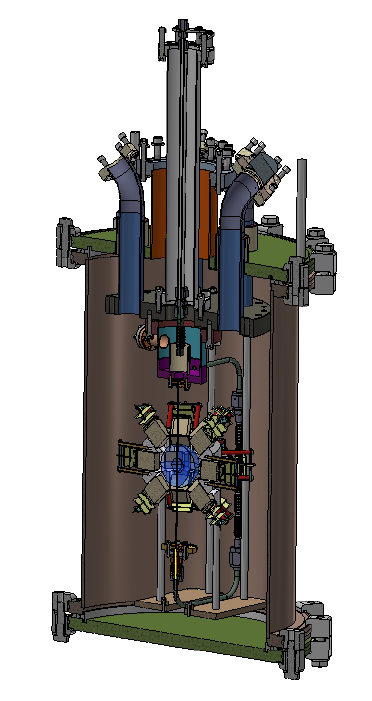
\includegraphics[width=0.75\textwidth , height=0.3\textheight]{detCAD.png}% Here is how to import 
\end{subfigure}	
\begin{subfigure}[c]{0.45\textwidth}
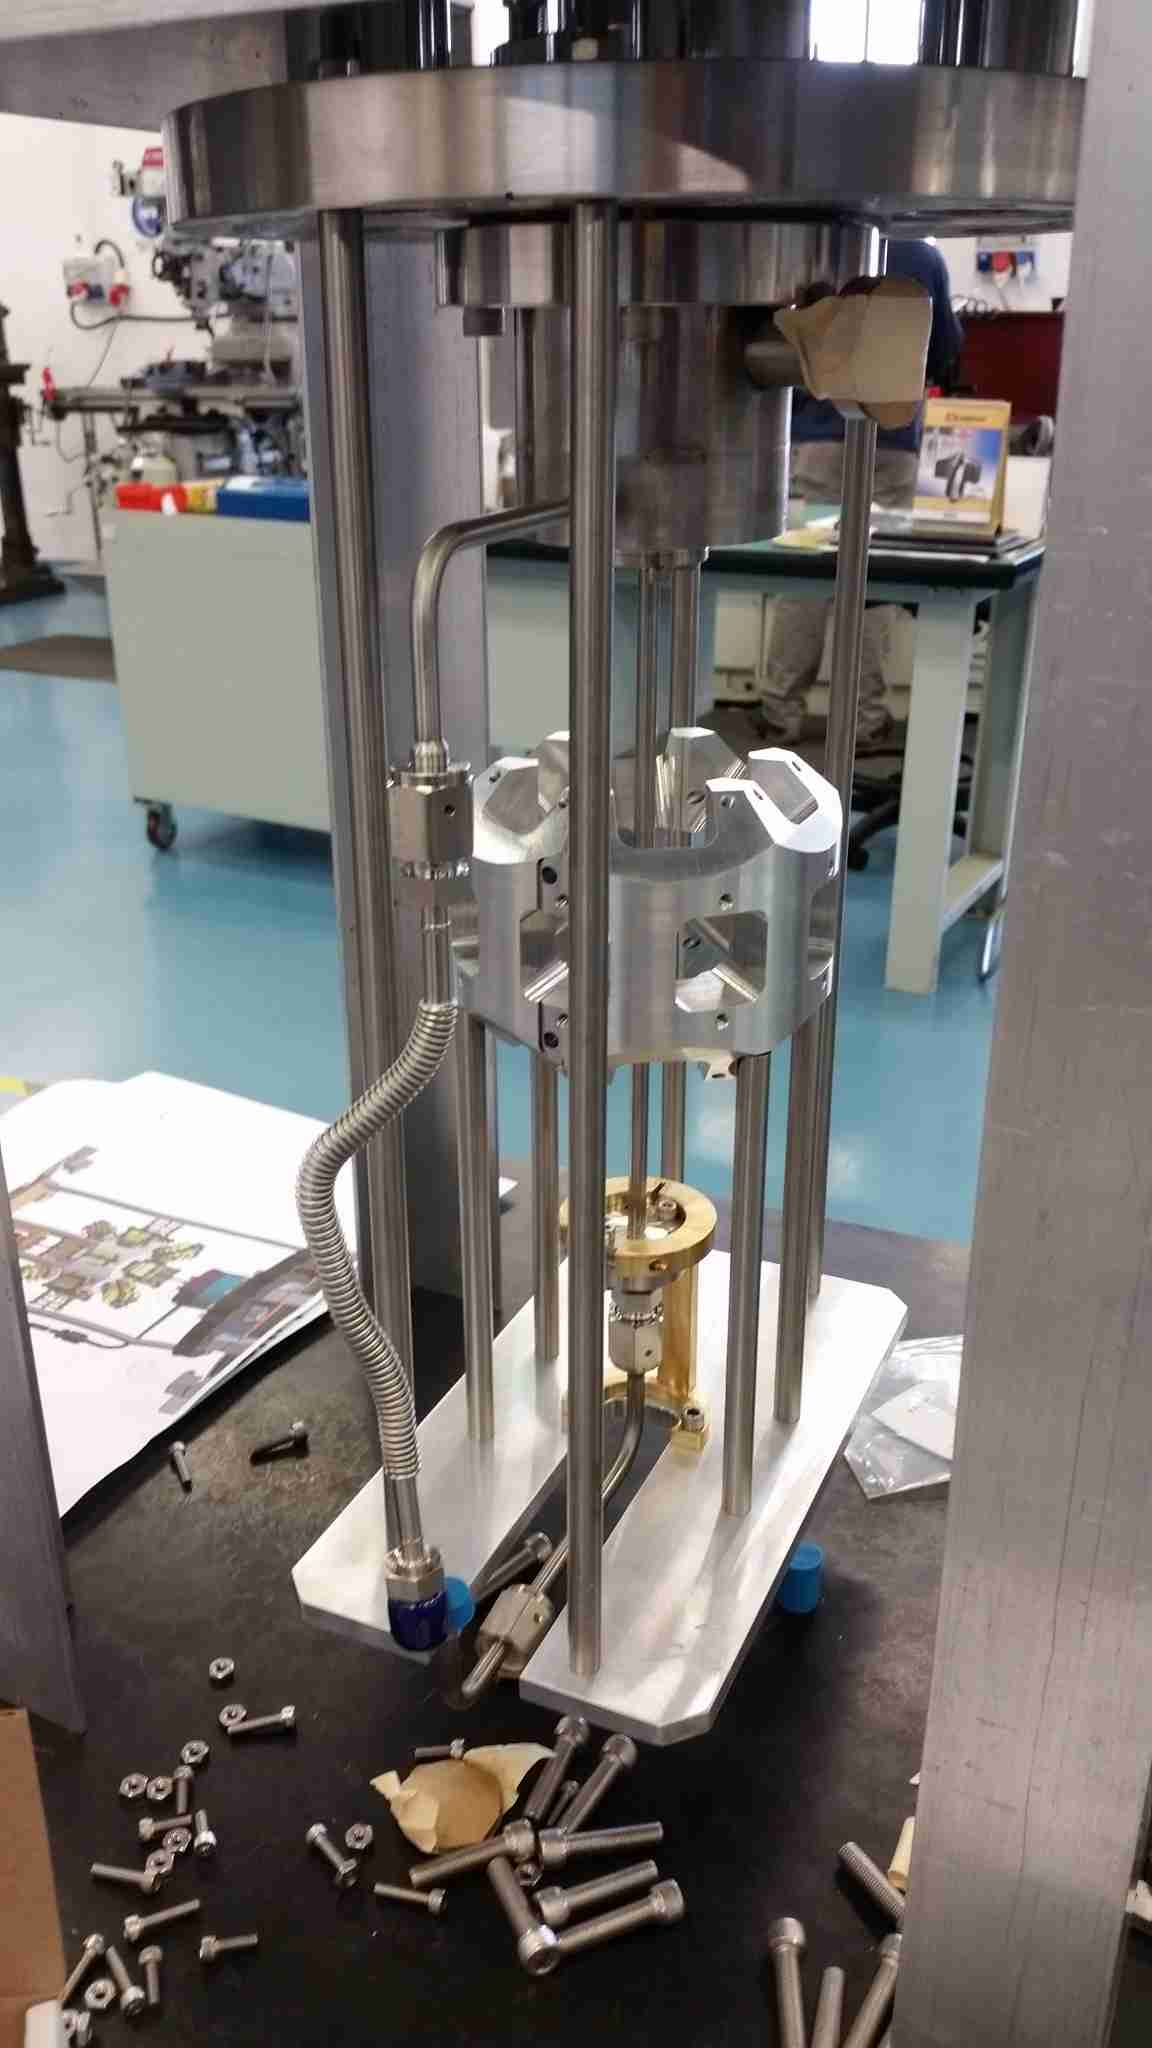
\includegraphics[width=\textwidth , height=0.3\textheight]{detReal_small.jpg}% Here is how to import 
\end{subfigure}	
\caption{\label{fig:detector} (Left) CAD design of the detector part. (Right) First mounting of the 
detector part, still not connected to the rest of the system.}
\end{figure}
%%%%%%%%%%%%%%%%%%%%%%%%%%%%%%%%%%%%%%%%%%%%%%%%%%%%%%%%%%%%%%%%%%%%%%%%%%%%
